\documentclass{article}
\usepackage[T1]{fontenc}
\usepackage{lmodern}
\usepackage{graphicx}
\usepackage{amsmath,amssymb}
\usepackage[a4paper,margin=2cm]{geometry}
\usepackage[absolute,overlay]{textpos}
\setlength{\TPHorizModule}{1mm}
\setlength{\TPVertModule}{1mm}
\usepackage[indonesian]{babel}
\usepackage{hyperref}
\setlength{\emergencystretch}{2em}
% unit: Halaman 16

\begin{document}

% === Halaman 16 (llm) ===

\begin{itemize}
    \item Contoh: Bentuklah tabel perkalian untuk GF(11), kemudian tentukan solusi untuk $x^2 \equiv 5 \pmod{11}$
\end{itemize}

\vspace{10mm}

\begin{align*}
    & x^2 \equiv 5 \pmod{11} \\
    & \text{Maka:} \\
    & x^2 = 16 \rightarrow x_1 = 4 \\
    & x^2 = 49 \rightarrow x_2 = 7
\end{align*}

\vspace{5mm}

Cara lain: cari elemen diagonal $= 5$, lalu ambil elemen mendatar atau elemen Vertikalnya (dilingkari).

\vspace{10mm}

\textcolor{red}{Sumber: Andreas Steffen, Elliptic Curve Cryptography} \\
\text{Rinaldi Munir/L4021 Kriptografi}

% deskripsi: Tabel perkalian Galois Field GF(11) dengan penandaan warna dan lingkaran untuk menunjukkan solusi x^2 = 5 mod 11.
% bbox normalisasi: [0.1800, 0.2300, 0.6100, 0.8800]
\begin{textblock*}{90.30mm}(37.80mm,68.31mm)
\noindent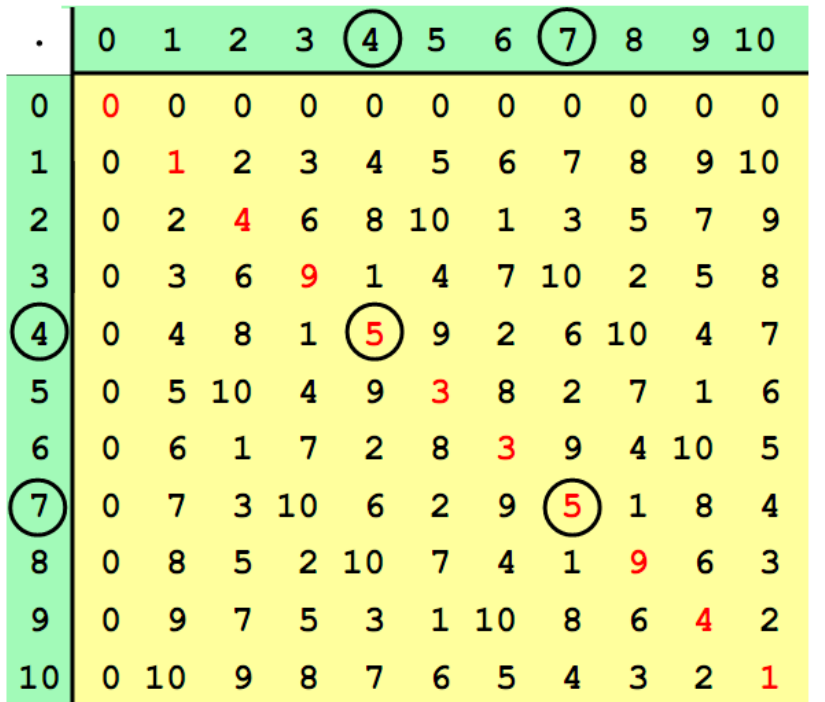
\includegraphics[width=90.30mm,height=193.05mm]{../../images/llm/page_016_img_01.png}%
\end{textblock*}

\end{document}
